\section{Planning and Paperwork}

\index{mapping software!Trailforks}
The \pbproleref{role:race_org_team} should prepare a few potential routes for each event,
typically using software like Trailforks or MapMyRide as shown in \reffig{road_pbp_trailforks}.

\pbproleref{role:local_teams} can assist the primary organizing organization with their local knowledge of roads and venues.

\begin{figure}[h]
  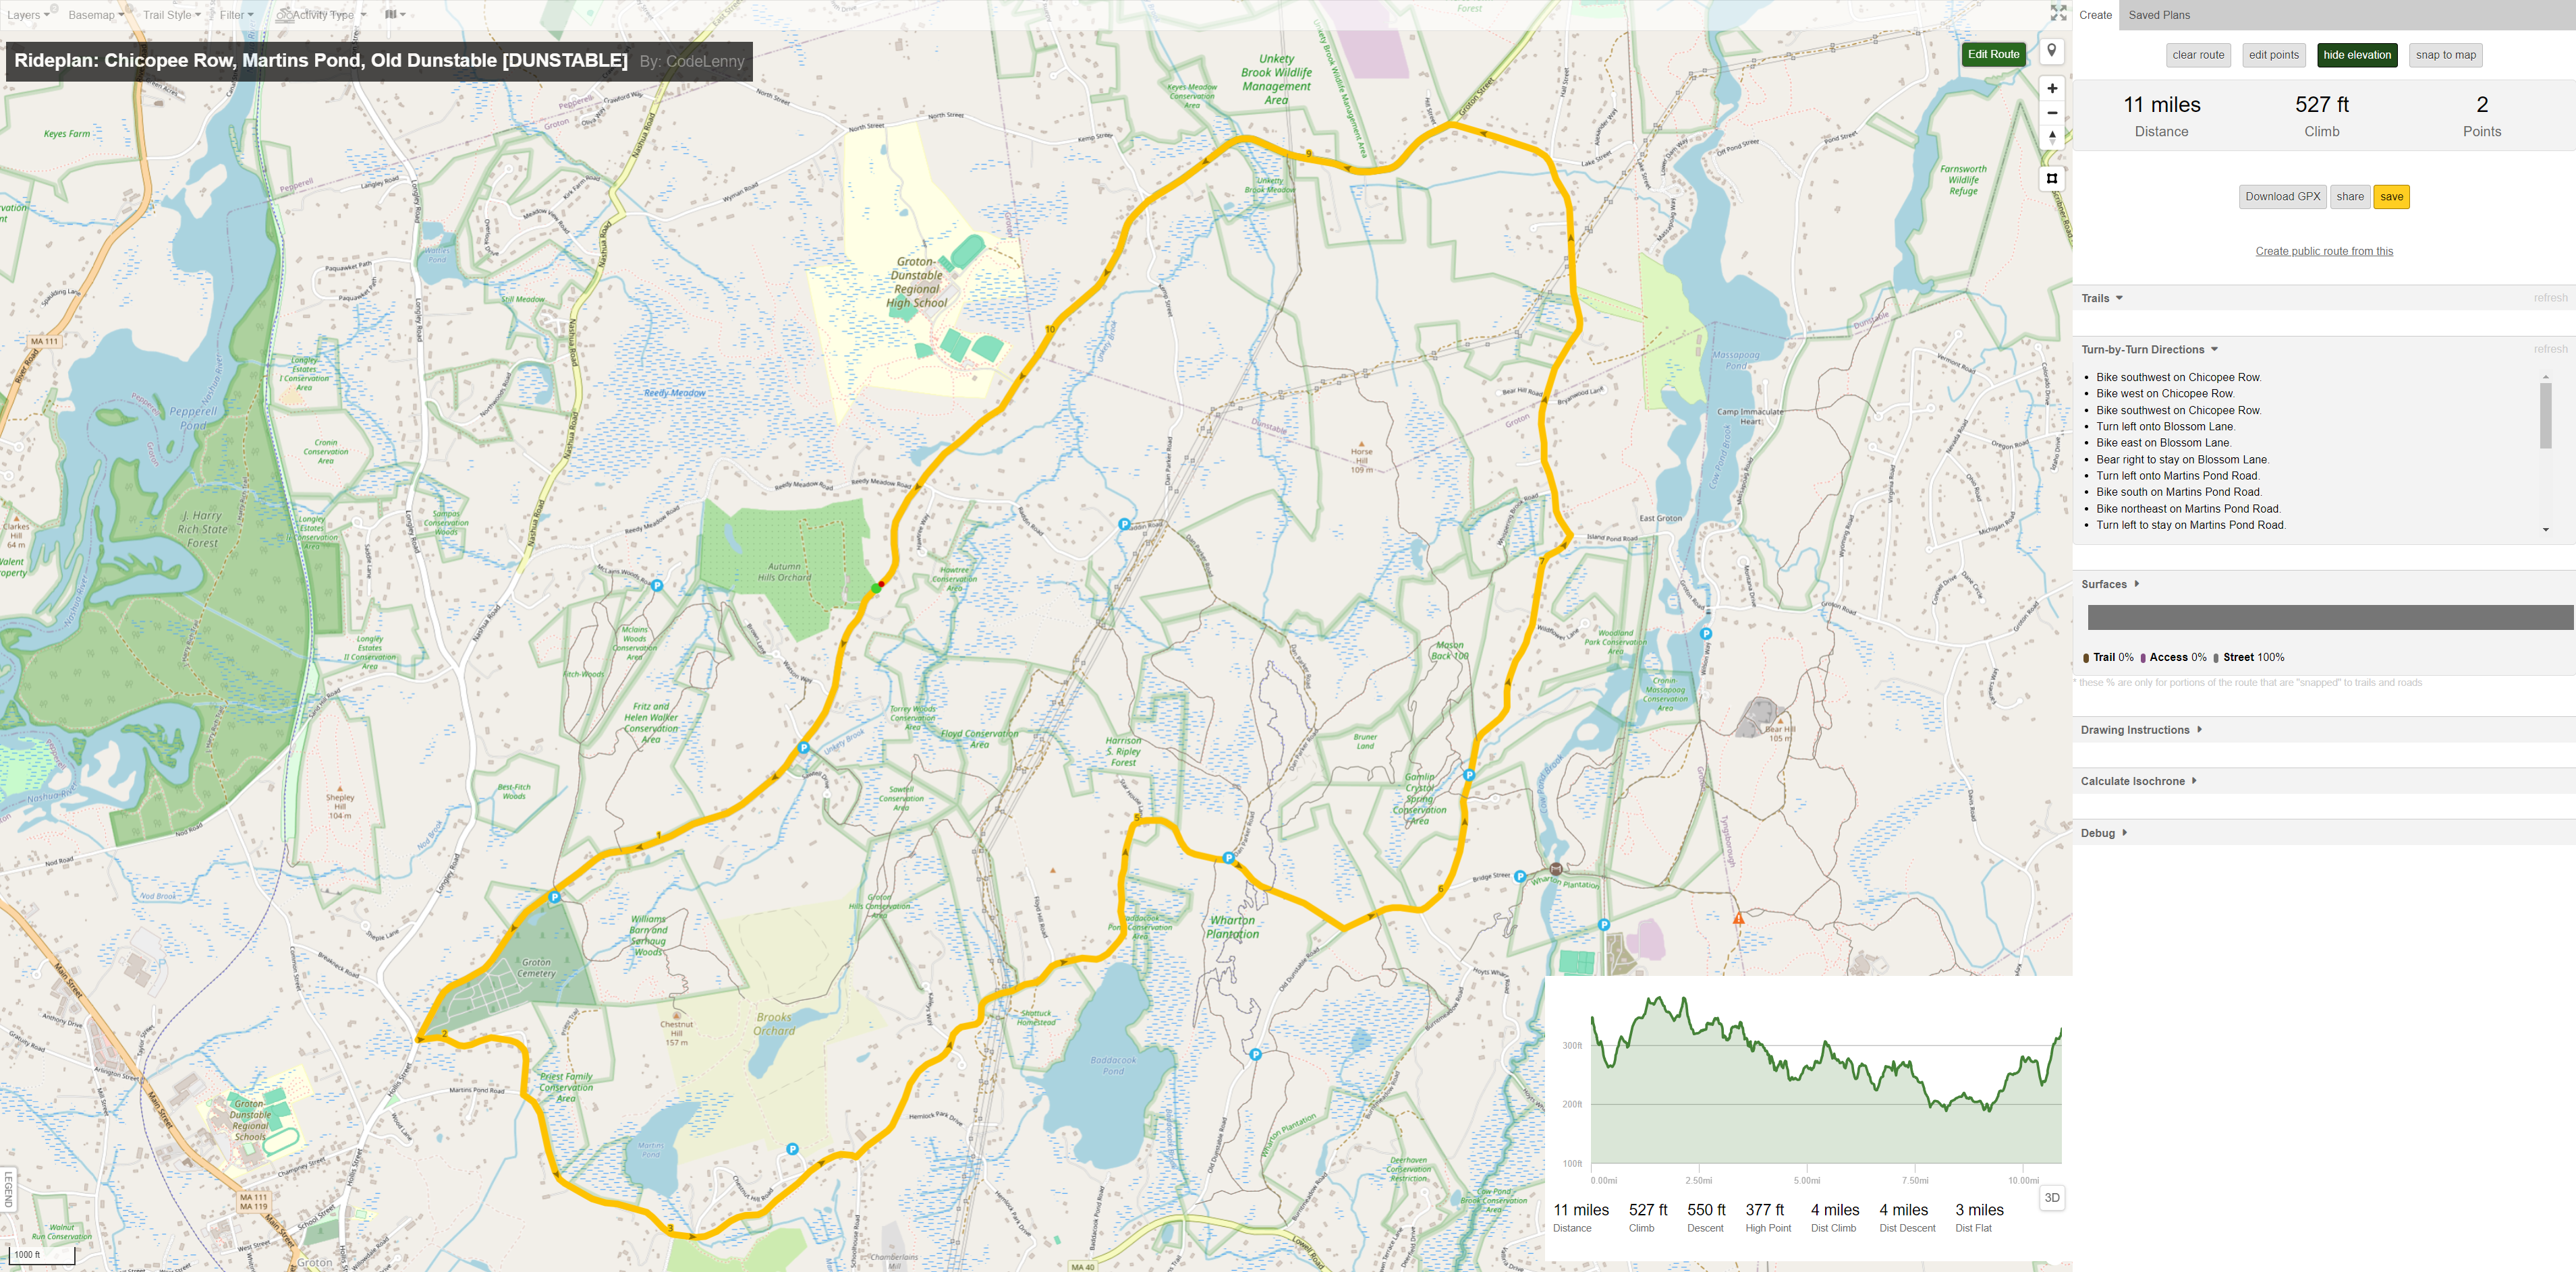
\includegraphics[width=1\textwidth]{2024_groton_trailforks.png}
  \caption[Road race course map in Trailforks]{
    A potential road race course in Groton, MA
    prepared via Trailforks for the 2024 Road Season.\\
    Credit: Flyyn Leonard}
  \labfig{road_pbp_trailforks}
\end{figure}


The \pbproleref{role:lead_org} should contact the local town or city
to determine what permits may be required, and make an initial contact to the police department,
as the police are typically a critical component to planning and running the race.

Once the race has passed the initial hurdle of getting a route and hasn't been shot down by the local government,
the \pbproleref{role:race_org_team} should evaluate local services and get quotes for:

\begin{itemize}
  \item Medical coverage, often by a local fire department or contracted private ambulance service
  \item Barriers and other course supplies - these may be supplied by the local police or highway department, or rented from private companies
  \item Additional venues for parking and staging (described in more detail below)
\end{itemize}

The \pbproleref{role:eccc_coordination_team} is available to help and advise the organizing team throughout this entire process,
and can often provide suggestions of who to contact, and have a list of departments and private companies that have been used in the past.

\subsubsection{Additional Venues}

Along with the on-road courses, you will need to plan where riders will park,
an area where an intro-clinic can be held (for criterium days),
a place to setup registration,
a finish line,
and an area by the course for staging.

These locations may all be in one large parking lot, or multiple smaller venues can be used.

Many ECCC races have had good luck contacting local K-12 schools, which are typically available for the weekend.

\subsection{Budget}

Using all of the information gathered in the initial planning phase, the \pbproleref{role:race_org_team} should start drafting a race budget
to ensure the race will be financially viable.

This budget can also serve as a to-do list, reminding organizers of the various services that will need to be contracted for the event.

A sample budget is included in \nrefch{event_budget}, and teams can contact the \pbproleref{role:eccc_coordination_team}
for a digital copy of the ECCC race budget template.
Using the official ECCC budget format is preferred, allowing ECCC staff to easily compile and compare budgets across weekends and years.

Teams should contact the \pbproleref{role:eccc_coordination_team} to discuss what registration fees should be for the entire season -
the ECCC tries to keep registration fees consistent across all races of the season, which makes it easy for teams to register.

\subsection{Flyer Design}

\begin{marginfigure}
  \includegraphics{2022_ship_scurry_flyer_pg1.png}
  \caption[An example race flyer]{A race flyer with the standard USA Cycling/ECCC formatted event schedule, from the 2022 Shipensburg Scurry}
  \labfig{road_pbp_flyer}
\end{marginfigure}

Once the race is deemed viable, the \pbproleref{role:race_org_team} should prepare a flyer, working with the \pbproleref{role:eccc_coordination_team}
to ensure the flyer meets the standard format dictated by the USA Cycling permitting process as well as the ECCC standards.

Race flyers should include:
\begin{itemize}
  \item The event schedule (in a USA Cycling approved format)
  \item Course maps for each event
  \item The address(es) of the race venue(s)
  \item The registration fees (noting day-of surcharges and student discounts)
  \item The methods of registration, including online (BikeReg), collegiate team bulk registration, and in-person day-of registration
  \item The deadlines for registering
  \item Driving directions (and other forms of transportation if applicable, such as public transportation)
  \item The type and format of contracted medical standby services, and the address of the nearest hospital for each venue
\end{itemize}

The race flyer is critical to obtaining a USA Cycling event permit.

\subsection[USA Cycling Permitting]{Obtaining a USA Cycling Permit}

Working with the \pbproleref{role:eccc_coordination_team}, the \pbproleref{role:lead_org} should submit a USA Cycling event permit application.

Once approved, this will provide Certificates of Insurance (COI) % TODO: add to glossary
that are typically required by the local government and venues,
and should automatically start the process of getting USA Cycling Officials to work the event.

\begin{marginfigure}
  \includegraphics{2024_usac_permit_application.png}
  \caption{USA Cycling event permit application form}
  \labfig{road_pbp_usac_permit_app}
\end{marginfigure}

\subsection{Additional Planning}

Along with all the essential items above, there's additional items that need to be coordinated.

\subsubsection{Marketing and Sponsorship}

The current collegiate turnout to a race weekend will likely not generate enough registration funds to balance your budget.
Most ECCC races use two key elements to balance the budget: advertising race fields for non-collegiate riders, and getting sponsorship.

The \pbproleref{role:lead_org} should consider the existing connections to sponsors that they may be able to request event-specific sponsorship from,
and should also evaluate if there are local businesses, such as bike shops or banks that might sponsor the event.

\pbproleref{role:local_teams} can be a huge assistance finding local media and other marketing opportunities, and could contact their team sponsors
in case the sponsors might be interested in sponsoring the event.

\subsubsection{Online Registration}

The \pbproleref{role:eccc_season_coordinator} will work with the \pbproleref{role:lead_org} to setup BikeReg pages for the event,
traditionally using the ECCC's BikeReg account.

\subsubsection{Volunteer Signup}

The \pbproleref{role:primary_promoter} should work with the \pbproleref{role:assistant_promoter} to ensure that all volunteer positions will be filled,
including lead/follow cars and drivers, and course marshalling.

Typically the promoters will reach out to \pbproleref{role:local_teams} to find volunteers.

\subsubsection{Food Planning}

The ECCC expects that the \pbproleref{role:lead_org} will plan to feed the officials, medical staff, and the \pbproleref{role:race_ops_team}.
% TODO: document this expectation as a regulation (in the rules section), and link to the regulation
Additionally, races typically provide some food for marshals as a thank-you (often in the form of pizza).
